\documentclass[12pt]{book} % Change to book
\usepackage{amsmath} % for mathematical expressions
\usepackage{xcolor} % for colored text
\usepackage{graphicx} % for including images
\usepackage{url}
\usepackage{booktabs} % for better-looking tables
\usepackage{makecell}
\usepackage{indentfirst}
\usepackage{algorithm}
\usepackage{algpseudocode}
\usepackage{amssymb}
\usepackage{placeins} % For \FloatBarrier
\usepackage{listings}
% Define the language style for Python code
\lstset{
    language=Python,
    basicstyle=\ttfamily,
    keywordstyle=\color{blue},
    stringstyle=\color{red},
    commentstyle=\color{gray},
    morecomment=[l][\color{magenta}]{\#},
    frame=single,
    breaklines=true
}
\begin{document}
\chapter{Network Flow}

\section{Introduction to Network Flow}

\subsection{Definitions and Key Concepts}

Network flow studies how resources move through networks, which consist of nodes connected by edges. Each edge has a capacity limiting the flow it can carry. The primary goal in network flow problems is optimizing this flow to meet various constraints efficiently.

\textbf{Key Terms:}
- \textbf{Flow:} The amount passing through an edge, denoted by \( f(u, v) \) for flow from node \( u \) to \( v \).
- \textbf{Capacity:} Maximum flow an edge can handle, denoted by \( c(u, v) \).
- \textbf{Residual Capacity:} Remaining capacity after current flow is considered, denoted by \( c_f(u, v) \).
- \textbf{Source and Sink:} The start (source) and end (sink) points in a flow network.

\subsection{Importance of Network Flow}

Network flow algorithms address numerous practical problems across diverse domains:
- \textbf{Transportation Planning:} Optimizing traffic flows and resource allocation in transportation networks.
- \textbf{Network Routing:} Efficient data packet routing in computer networks to enhance communication.
- \textbf{Supply Chain Management:} Optimizing goods flow from production to consumption, minimizing costs and enhancing efficiency.
- \textbf{Telecommunications:} Managing data flow to maximize bandwidth usage and improve service quality.

\subsection{Historical Overview and Applications}

The concept of network flow has been a focal point of study since the mid-20th century, propelled by foundational work from researchers like Ford and Fulkerson.

\textbf{Ford-Fulkerson Algorithm:}
Developed in 1956, this algorithm is pivotal for calculating maximum flows. It repetitively identifies paths from the source to the sink where additional flow is possible (augmenting paths) and enhances the flow until no further such paths exist.

\textbf{Applications:}
- \textbf{Transportation Networks:} Used to streamline traffic and enhance routing efficiency.
- \textbf{Computer Networks:} Applies to routing and bandwidth management, ensuring efficient network operations.
- \textbf{Supply Chains and Telecommunications:} Optimizes logistics and data transmission paths, improving overall network efficiency and cost-effectiveness.

This exploration underscores the integral role of network flow in tackling complex optimization challenges across various sectors, highlighting its enduring relevance and potential for future technological advancements.


\FloatBarrier
\subsubsection{Ford-Fulkerson Algorithm}
The Ford-Fulkerson algorithm is a classic method for computing the maximum flow in a flow network. It operates by iteratively finding augmenting paths from the source to the sink and updating the flow along these paths until no more augmenting paths exist.

The following algorithm implements the Ford-Fulkerson algorithm for finding the maximum flow in a flow network:
\FloatBarrier
\begin{algorithm}
\caption{Ford-Fulkerson Algorithm}\label{ford-fulkerson}
\begin{algorithmic}[1]
\Function{FordFulkerson}{$graph, source, sink$}
    \State $residual\_graph \gets$ \Call{ConstructResidualGraph}{$graph$}
    \State $max\_flow \gets 0$
    \While{\textbf{True}}
        \State $augmenting\_path \gets$ \Call{FindAugmentingPath}{$residual\_graph, source, sink$}
        \If{$augmenting\_path$ is \textbf{None}}
            \State \textbf{break}
        \EndIf
        \State $max\_flow \mathrel{+}= $ \Call{AugmentFlow}{$residual\_graph, augmenting\_path$}
    \EndWhile
    \State \textbf{return} $max\_flow$
\EndFunction
\end{algorithmic}
\end{algorithm}
\FloatBarrier
\textbf{Explanation:}
\begin{itemize}
    \item The \texttt{FordFulkerson} function implements the Ford-Fulkerson algorithm for finding the maximum flow in a flow network.
    \item It constructs the residual graph from the given graph using the \texttt{ConstructResidualGraph} function.
    \item It initializes the maximum flow to 0 and iterates until no more augmenting paths can be found in the residual graph.
    \item In each iteration, it finds an augmenting path using the \texttt{FindAugmentingPath} function.
    \item If no augmenting path is found, the algorithm terminates.
    \item Otherwise, it augments the flow along the augmenting path using the \texttt{AugmentFlow} function and updates the maximum flow.
    \item Finally, it returns the maximum flow computed.
\end{itemize}

This algorithm efficiently computes the maximum flow in a flow network using the Ford-Fulkerson algorithm.

The key steps of the Ford-Fulkerson algorithm include:
\begin{enumerate}
    \item Initializing the flow to zero.
    \item Finding augmenting paths from the source to the sink in the residual graph.
    \item Determining the maximum flow that can be pushed along each augmenting path.
    \item Updating the flow by augmenting it with the maximum flow along each path.
    \item Repeat steps 2-4 until no more augmenting paths exist.
\end{enumerate}

\FloatBarrier
\subsubsection{Residual Graph}
The residual graph plays a crucial role in the Ford-Fulkerson algorithm. It represents the remaining capacity available for flow along each edge after accounting for the flow already sent through the edge.

\textbf{Residual Capacity:} The residual capacity \( c_f(u, v) \) of an edge \( (u, v) \) in the residual graph is defined as:
\[ c_f(u, v) = c(u, v) - f(u, v) \]
where \( c(u, v) \) is the capacity of the edge and \( f(u, v) \) is the flow along the edge.

\textbf{Residual Graph Construction:} Given a flow network and its corresponding flow, the residual graph can be constructed by adding edges to represent the residual capacities. For each edge \( (u, v) \) with flow \( f(u, v) \) and capacity \( c(u, v) \), two edges are added to the residual graph: \( (u, v) \) with residual capacity \( c_f(u, v) \) and \( (v, u) \) with residual capacity \( f(u, v) \).

\FloatBarrier
\subsubsection{Python Implementation}
Here's a Python implementation of the Ford-Fulkerson algorithm:
\FloatBarrier
\begin{lstlisting}
def ford_fulkerson(graph, source, sink):
    residual_graph = construct_residual_graph(graph)
    max_flow = 0
    while True:
        augmenting_path = find_augmenting_path(residual_graph, source, sink)
        if augmenting_path is None:
            break
        max_flow += augment_flow(residual_graph, augmenting_path)
    return max_flow
\end{lstlisting}
\FloatBarrier
\textbf{Example}
Consider the following flow network:

\FloatBarrier
\begin{figure}[h]
    \centering
    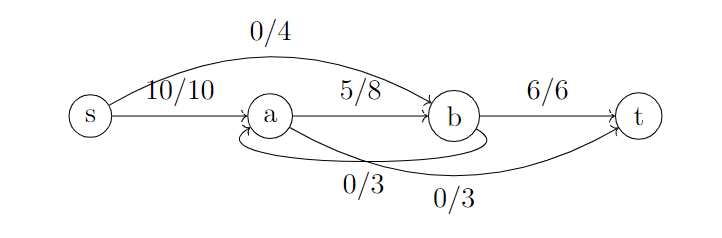
\includegraphics[width=0.6\textwidth]{images/Example_flow_network.png}
    \caption{Example Flow Network}
\end{figure}
\FloatBarrier

Using the Ford-Fulkerson algorithm, we can compute the maximum flow in this network, which is 11 units.


\section{Fundamentals of Network Flow}

Network flow theory is a branch of graph theory that deals with the study of flows in networks. In this section, we will cover the basic concepts and terminology related to network flow.

\subsection{Graphs and Networks}

In network flow theory, a \textbf{graph} \(G\) is a mathematical structure consisting of a set of vertices \(V\) and a set of edges \(E\), where each edge connects two vertices. 

A \textbf{network} is a directed graph \(G = (V, E)\) with two distinguished vertices: a \textbf{source} vertex \(s\) and a \textbf{sink} vertex \(t\). The source vertex represents the origin of flow, while the sink vertex represents the destination.

\subsection{Flow Networks and Capacity}

A \textbf{flow network} is a directed graph \(G = (V, E)\) with a capacity function \(c : E \rightarrow \mathbb{R}^+\) that specifies the maximum amount of flow that can be sent through each edge.

Formally, a flow network consists of:
\begin{itemize}
    \item A set of vertices \(V\).
    \item A set of directed edges \(E\), where each edge \((u, v) \in E\) has a capacity \(c(u, v)\).
    \item A source vertex \(s\) and a sink vertex \(t\).
\end{itemize}

\subsection{Types of Flow Problems}

There are several types of flow problems that can be solved using network flow algorithms:

\begin{enumerate}
    \item \textbf{Maximum Flow}: The goal is to find the maximum amount of flow that can be sent from the source to the sink in a flow network.
    \item \textbf{Minimum Cut}: The goal is to find the minimum capacity cut that separates the source from the sink in a flow network.
    \item \textbf{Multi-Commodity Flow}: The goal is to send multiple commodities (types of flow) from various sources to various sinks, subject to capacity constraints.
    \item \textbf{Network Design}: The goal is to design a network (e.g., transportation network, telecommunication network) to optimize certain objectives such as minimizing costs or maximizing throughput.
\end{enumerate}


Let's consider the problem of finding the maximum flow in a flow network using the Ford-Fulkerson algorithm.

\textbf{Algorithm Description}

The Ford-Fulkerson algorithm is an iterative method for finding the maximum flow in a flow network. It operates by repeatedly augmenting the flow along augmenting paths from the source to the sink until no more augmenting paths exist.
\FloatBarrier
\begin{algorithm}[H]
\caption{Ford-Fulkerson Algorithm}
\begin{algorithmic}[1]
\State Initialize flow on all edges to 0
\While{there exists an augmenting path from $s$ to $t$}
    \State Find an augmenting path $p$ from $s$ to $t$
    \State Compute the residual capacity $c_f(p)$ of $p$
    \State Augment flow along $p$ by $c_f(p)$
\EndWhile
\end{algorithmic}
\end{algorithm}
\FloatBarrier
\textbf{Mathematical Detail}

Let \(f(u, v)\) denote the flow along edge \((u, v)\) in the flow network, and let \(c(u, v)\) denote the capacity of edge \((u, v)\). The residual capacity \(c_f(u, v)\) of edge \((u, v)\) after flow \(f\) has been added is given by:
\[ c_f(u, v) = c(u, v) - f(u, v) \]

An \textbf{augmenting path} is a simple path from the source \(s\) to the sink \(t\) in the residual graph \(G_f\), where the residual capacity of each edge along the path is positive. The \textbf{residual graph} \(G_f\) is the graph that represents the remaining capacity on each edge after the flow \(f\) has been added to the original flow network \(G\).

\textbf{Python Implementation}

Here's a Python implementation of the Ford-Fulkerson algorithm:
\FloatBarrier
\begin{lstlisting}
def ford_fulkerson(graph, source, sink):
    flow = {(u, v): 0 for u, v in graph.edges()}
    residual_capacity = {(u, v): graph[u][v]['capacity'] for u, v in graph.edges()}
    
    def dfs(s, t, path):
        if s == t:
            return path
        for neighbor in graph.neighbors(s):
            if residual_capacity[s, neighbor] > 0 and (s, neighbor) not in path:
                augmenting_path = dfs(neighbor, t, path + [(s, neighbor)])
                if augmenting_path:
                    return augmenting_path
        return None
    
    augmenting_path = dfs(source, sink, [])
    while augmenting_path:
        residual_capacity_path = min(residual_capacity[u, v] for u, v in augmenting_path)
        for u, v in augmenting_path:
            flow[u, v] += residual_capacity_path
            flow[v, u] -= residual_capacity_path
            residual_capacity[u, v] -= residual_capacity_path
            residual_capacity[v, u] += residual_capacity_path
        augmenting_path = dfs(source, sink, [])
    
    return sum(flow[source, v] for v in graph.neighbors(source))
\end{lstlisting}

\section{Maximum Flow Theory}

\subsection{The Max-Flow Min-Cut Theorem}

The Max-Flow Min-Cut Theorem is a fundamental result in network flow theory that establishes a duality between maximum flows and minimum cuts in a flow network. 

\textbf{Theorem:} In any flow network, the value of the maximum flow is equal to the capacity of the minimum cut.

This theorem provides a powerful insight into the structure of flow networks and is the basis for many algorithms for solving the maximum flow problem.


\subsubsection{Example: Ford-Fulkerson Algorithm}

Let's consider a simple example of a flow network and apply the Ford-Fulkerson algorithm to find the maximum flow.

\FloatBarrier
\begin{figure}[h]
    \centering
    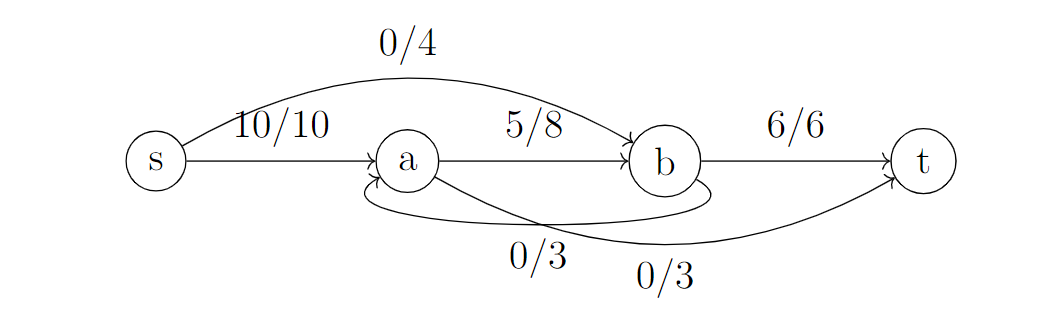
\includegraphics[width=0.6\textwidth]{images/Visualization_of_Ford_Fulkerson_Algorithm.png}
    \caption{Visualization of the Push-Relabel Algorithm}
\end{figure}
\FloatBarrier

\textbf{Algorithm: Ford-Fulkerson}

\begin{algorithm}[H]
\caption{Ford-Fulkerson Algorithm}\label{alg:ford-fulkerson}
\begin{algorithmic}[1]
\State Initialize flow $f$ to 0
\While{there exists an augmenting path $p$}
    \State Find the residual capacity $c_f(p)$ of path $p$
    \State Augment flow $f$ along path $p$ by $c_f(p)$
\EndWhile
\end{algorithmic}
\end{algorithm}

\textbf{Mathematical Detail:}

The residual capacity $c_f(p)$ of an augmenting path $p$ is the minimum capacity of any edge along the path $p$. Augmenting flow along path $p$ involves increasing the flow along each edge by $c_f(p)$.

\FloatBarrier
\begin{lstlisting}
def ford_fulkerson(graph, source, sink):
    residual_graph = initialize_residual_graph(graph)
    max_flow = 0
    while True:
        path = find_augmenting_path(residual_graph, source, sink)
        if not path:
            break
        augment(residual_graph, path)
        max_flow += path_flow
    return max_flow
\end{lstlisting}
\FloatBarrier

\subsection{Path Augmentation}

Path augmentation is a fundamental technique used in various algorithms for finding maximum flows in network flow problems.

\subsubsection{Example: Edmonds-Karp Algorithm}

The Edmonds-Karp algorithm is a variation of the Ford-Fulkerson algorithm that uses BFS to find augmenting paths, ensuring that the shortest augmenting path is always chosen.

\textbf{Algorithm: Edmonds-Karp}
\FloatBarrier
\begin{algorithm}[H]
\caption{Edmonds-Karp Algorithm}\label{alg:edmonds-karp}
\begin{algorithmic}[1]
\State Initialize flow $f$ to 0
\While{there exists a shortest augmenting path $p$ from $s$ to $t$}
    \State Find the residual capacity $c_f(p)$ of path $p$
    \State Augment flow $f$ along path $p$ by $c_f(p)$
\EndWhile
\end{algorithmic}
\end{algorithm}
\FloatBarrier
\textbf{Mathematical Detail:}

The shortest augmenting path $p$ is found using BFS. The residual capacity $c_f(p)$ of path $p$ is the minimum capacity of any edge along the path. Augmenting flow along path $p$ involves increasing the flow along each edge by $c_f(p)$.

\FloatBarrier
\begin{lstlisting}
def edmonds_karp(graph, source, sink):
    residual_graph = initialize_residual_graph(graph)
    max_flow = 0
    while True:
        path = find_shortest_augmenting_path(residual_graph, source, sink)
        if not path:
            break
        augment(residual_graph, path)
        max_flow += path_flow
    return max_flow
\end{lstlisting}
\FloatBarrier

\subsection{Capacity Scaling}

Capacity scaling is an optimization technique used to improve the efficiency of flow algorithms by gradually increasing the capacities of the edges in the flow network.

\subsubsection{Example: Capacity Scaling Algorithm}

The Capacity Scaling algorithm is an extension of the Ford-Fulkerson algorithm that incorporates capacity scaling to improve performance.

\textbf{Algorithm: Capacity Scaling}
\FloatBarrier
\begin{algorithm}[H]
\caption{Capacity Scaling Algorithm}\label{alg:capacity-scaling}
\begin{algorithmic}[1]
\State Initialize scaling factor $f$ to a large value
\State Reduce capacities in the graph to be less than $f$
\State Initialize flow $f$ to 0
\While{there exists an augmenting path $p$}
    \State Find the residual capacity $c_f(p)$ of path $p$
    \State Augment flow $f$ along path $p$ by $c_f(p)$
\EndWhile
\end{algorithmic}
\end{algorithm}
\FloatBarrier
\textbf{Mathematical Detail:}

The scaling factor $f$ determines the minimum capacity of any edge in the graph. Initially, $f$ is set to a large value, and capacities in the graph are reduced to be less than $f$. This ensures that only significant edges are considered during the flow augmentation process.

\FloatBarrier
\begin{lstlisting}
def capacity_scaling(graph, source, sink):
    scaling_factor = calculate_scaling_factor(graph)
    reduce_capacities(graph, scaling_factor)
    max_flow = ford_fulkerson(graph, source, sink)
    return max_flow
\end{lstlisting}
\FloatBarrier

\section{Algorithms for Maximum Flow}

\subsection{The Ford-Fulkerson Algorithm}

\subsubsection{Algorithm Description}

The Ford-Fulkerson algorithm is a method for computing the maximum flow in a flow network. It operates by repeatedly augmenting the flow along a path from the source to the sink until no such path exists. The key idea is to find augmenting paths with residual capacity and increase the flow along these paths.

Let $G=(V, E)$ be a flow network with a source $s$ and a sink $t$. Let $c(u, v)$ be the capacity of edge $(u, v)$. The residual capacity $c_f(u, v)$ of edge $(u, v)$ is defined as $c(u, v) - f(u, v)$, where $f(u, v)$ is the flow along edge $(u, v)$.

The algorithm can be described as follows:
\FloatBarrier
\begin{algorithm}
\caption{Ford-Fulkerson Algorithm}
\begin{algorithmic}[1]
\Function{FordFulkerson}{$G, s, t$}
    \State Initialize flow $f(u, v)$ to 0 for all edges $(u, v) \in E$
    \While{there exists an augmenting path $p$ from $s$ to $t$ in $G_f$}
        \State Find the residual capacity $c_f(p)$ of path $p$
        \State Augment flow $f$ along path $p$ by $c_f(p)$
    \EndWhile
    \State \textbf{return} $f$
\EndFunction
\end{algorithmic}
\end{algorithm}
\FloatBarrier
Here, $G_f$ is the residual graph at each iteration, obtained by updating the capacities based on the current flow.

\textbf{Python Code Implementation:}
\FloatBarrier
\begin{lstlisting}
def ford_fulkerson(G, s, t):
    # Initialize flow f(u, v) to 0 for all edges (u, v) in E
    f = {}
    for u in G.keys():
        for v in G[u].keys():
            f[(u, v)] = 0
    
    # Function to find an augmenting path from s to t in G_f
    def find_augmenting_path(G, s, t, f):
        visited = {node: False for node in G.keys()}
        parent = {}
        queue = [s]
        visited[s] = True
        while queue:
            u = queue.pop(0)
            for v in G[u].keys():
                if not visited[v] and G[u][v] - f[(u, v)] > 0:
                    parent[v] = u
                    visited[v] = True
                    queue.append(v)
                    if v == t:
                        path = []
                        while v != s:
                            path.append(v)
                            v = parent[v]
                        path.append(s)
                        return path[::-1]
        return None
    
    # Function to find the residual capacity cf(p) of path p
    def residual_capacity(G, f, path):
        residual_cap = float('inf')
        for i in range(len(path) - 1):
            u, v = path[i], path[i + 1]
            residual_cap = min(residual_cap, G[u][v] - f[(u, v)])
        return residual_cap
    
    # Augment flow f along path p by cf(p)
    def augment_flow(f, path, cf):
        for i in range(len(path) - 1):
            u, v = path[i], path[i + 1]
            f[(u, v)] += cf
            f[(v, u)] -= cf
    
    # Main algorithm loop
    while True:
        # Find an augmenting path p from s to t in G_f
        augmenting_path = find_augmenting_path(G, s, t, f)
        if augmenting_path is None:
            break
        # Find the residual capacity cf(p) of path p
        cf = residual_capacity(G, f, augmenting_path)
        # Augment flow f along path p by cf(p)
        augment_flow(f, augmenting_path, cf)
    
    return f

# Example usage:
# G = {node: {neighbor: capacity}}
# G = {'s': {'a': 10, 'b': 5},
#      'a': {'b': 15, 't': 10},
#      'b': {'c': 5, 't': 10},
#      'c': {'t': 10},
#      't': {}}
# s = 's'
# t = 't'
# print(ford_fulkerson(G, s, t))
\end{lstlisting}

\subsubsection{Example Applications}

The Ford-Fulkerson algorithm has various applications, including:

\begin{itemize}
    \item Network flow optimization in transportation systems.
    \item Bandwidth allocation in communication networks.
    \item Resource allocation in project scheduling.
    \item Airline scheduling to maximize revenue.
\end{itemize}

\subsubsection{Limitations and Efficiency of the Ford-Fulkerson Algorithm}

The Ford-Fulkerson algorithm, while foundational in network flow analysis, exhibits certain limitations, particularly in complex or large-scale network scenarios:

\begin{enumerate}
    \item \textbf{Dependence on Augmenting Paths:} The algorithm's performance heavily relies on the choice of augmenting paths. Inefficient path selection can lead to exponential convergence times, especially if the paths increment flow minimally, resulting in numerous iterations.
    
    \item \textbf{Termination Issues:} The algorithm may fail to terminate if edge capacities are real numbers or if the residual graph contains negative cycles, potentially causing an infinite loop without reaching a maximum flow solution.
    
    \item \textbf{Scalability Challenges:} In large graphs with extensive vertices and edges, the algorithm's efficiency decreases due to the repetitive process of identifying augmenting paths, escalating the time complexity and rendering it impractical for large-scale applications.
    
    \item \textbf{Space Complexity:} Maintaining a residual graph for each iteration demands substantial memory, particularly in dense graphs, which can be prohibitive in environments with limited memory resources.
\end{enumerate}

While the Ford-Fulkerson algorithm is instrumental for smaller network flow problems, for larger or more complex networks, alternatives like the Push-Relabel or Dinic's algorithm may provide improved efficiency and scalability.


\subsection{The Push-Relabel Algorithm}

\subsubsection{Algorithm Overview}

The Push-Relabel algorithm is another approach to compute the maximum flow in a flow network. It maintains a preflow and iteratively pushes excess flow from high-priority nodes to low-priority nodes, gradually transforming it into a maximum flow.

Let $h(u)$ denote the height of node $u$, and $e(u)$ denote the excess flow at node $u$. The algorithm maintains a global height function $h$ and a labeling function $l$ to prioritize node selection for pushing excess flow.

The key operations in the algorithm are:

\begin{itemize}
    \item \textbf{Push operation:} Push excess flow from high-priority nodes to adjacent low-priority nodes.
    \item \textbf{Relabel operation:} Increase the height of a node to create a valid push opportunity.
\end{itemize}

The algorithm can be described as follows:

\begin{algorithm}
\caption{Push-Relabel Algorithm}
\begin{algorithmic}[1]
\Function{PushRelabel}{$G, s, t$}
    \State Initialize preflow and heights
    \While{there exists a node with excess flow}
        \State Push or relabel the node
    \EndWhile
    \State \textbf{return} maximum flow
\EndFunction
\end{algorithmic}
\end{algorithm}

\FloatBarrier
\textbf{Python Code Implementation:}
\FloatBarrier
\begin{lstlisting}
def push_relabel(G, s, t):
    # Initialize preflow and heights
    height = {node: 0 for node in G.keys()}
    preflow = {(u, v): 0 for u in G.keys() for v in G[u].keys()}
    excess = {node: 0 for node in G.keys()}
    height[s] = len(G)
    excess[s] = float('inf')
    for v in G[s].keys():
        preflow[(s, v)] = G[s][v]
        preflow[(v, s)] = -G[s][v]
        excess[v] = G[s][v]
    
    # Push operation
    def push(u, v):
        flow = min(excess[u], preflow[(u, v)])
        preflow[(u, v)] -= flow
        preflow[(v, u)] += flow
        excess[u] -= flow
        excess[v] += flow
    
    # Relabel operation
    def relabel(u):
        height[u] = min([height[v] for v in G[u].keys() if preflow[(u, v)] > 0]) + 1
    
    # Main algorithm loop
    while True:
        active_nodes = [node for node in G.keys() if node != s and node != t and excess[node] > 0]
        if not active_nodes:
            break
        for u in active_nodes:
            v = next(iter(G[u]))
            if height[u] == height[v] + 1:
                push(u, v)
            else:
                relabel(u)
    
    # Calculate maximum flow
    max_flow = sum(preflow[(s, v)] for v in G[s].keys())
    
    return max_flow

# Example usage:
# G = {node: {neighbor: capacity}}
# G = {'s': {'a': 10, 'b': 5},
#      'a': {'b': 15, 't': 10},
#      'b': {'c': 5, 't': 10},
#      'c': {'t': 10},
#      't': {}}
# s = 's'
# t = 't'
# print(push_relabel(G, s, t))
\end{lstlisting}

\subsubsection{Performance Analysis of the Push-Relabel Algorithm}

The Push-Relabel algorithm is distinguished by its efficiency and structured approach to solving network flow problems:

\begin{enumerate}
    \item \textbf{Time Complexity:} It achieves a worst-case time complexity of \(O(V^2E)\), where \(V\) and \(E\) are the number of vertices and edges, respectively. This is generally more favorable compared to the potentially exponential time complexity of the Ford-Fulkerson algorithm, particularly in large-scale networks.

    \item \textbf{Structured Flow Management:} The algorithm efficiently manages flow by maintaining a structured process of pushing and relabeling, which enhances performance and reduces unnecessary operations.

    \item \textbf{Optimizations:} Techniques like gap relabeling and global relabeling significantly improve convergence speeds, while strategic use of data structures like priority queues can optimize internal operations.
\end{enumerate}

Overall, the Push-Relabel algorithm combines theoretical rigor with practical efficiency, making it suitable for complex flow network challenges.

\subsubsection{Practical Implementations}

Effective implementation of the Push-Relabel algorithm involves several key considerations:

\begin{enumerate}
    \item \textbf{Data Structures:} Employing the right data structures, such as priority queues for node management, is crucial for efficient algorithm performance.

    \item \textbf{Algorithmic Optimizations:} Incorporating techniques like gap relabeling and discharge heuristics can significantly reduce the number of operations required and speed up the algorithm.

    \item \textbf{Parallelization:} Leveraging parallel computing can drastically reduce computation times, particularly beneficial for large network flows.

    \item \textbf{Robustness:} The algorithm should handle edge cases effectively, ensuring stability and accuracy, particularly in scenarios with complex network structures or unusual flow distributions.
\end{enumerate}

By addressing these practical aspects, the Push-Relabel algorithm can be optimized for robust and efficient performance across various real-world applications, delivering solutions that are both scalable and reliable.


\subsubsection{Dinic's Algorithm for Maximum Flow}

Dinic's algorithm is a robust method for determining the maximum flow in a network, employing level graphs and blocking flows to enhance computational efficiency.

\begin{itemize}
    \item \textbf{Level Graph:} A level graph is constructed from the residual network each iteration, representing vertices accessible from the source via the shortest path in terms of edge count.
    
    \item \textbf{Blocking Flow:} A blocking flow fully saturates paths from the source to the sink in the level graph, allowing significant increases in flow.
\end{itemize}

The algorithm progresses through the following steps:

\begin{enumerate}
    \item \textbf{Initialization:} Begin with zero flow and build the residual network from the initial capacities.
    
    \item \textbf{Construct Level Graph:} Use Breadth-First Search (BFS) to form a level graph, ensuring only the shortest paths are considered for subsequent flow augmentation.
    
    \item \textbf{Find Blocking Flow:} In the level graph, identify a blocking flow by saturating paths from the source to the sink, which maximizes flow incrementally.
    
    \item \textbf{Update Flow:} Apply the blocking flow to the original network, adjusting the flow along the paths utilized in the blocking flow, thereby increasing the overall flow.
    
    \item \textbf{Iterate:} Repeat the process of constructing level graphs and finding blocking flows until no further augmentations can be found, indicating the attainment of maximum flow.
\end{enumerate}

Dinic's algorithm is particularly effective due to its structured approach to augmenting flow, making it suitable for complex network flow problems with large datasets.


\textbf{Python Code}
\FloatBarrier
\begin{lstlisting}
    from collections import deque

def dinics_algorithm(graph, source, sink):
    def bfs():
        level = {source: 0}
        queue = deque([source])
        while queue:
            u = queue.popleft()
            for v, capacity in graph[u].items():
                if capacity > 0 and v not in level:
                    level[v] = level[u] + 1
                    queue.append(v)
        return level.get(sink, None)

    def dfs(u, flow):
        if u == sink:
            return flow
        for v, capacity in graph[u].items():
            if capacity > 0 and level[u] + 1 == level[v]:
                augmented_flow = dfs(v, min(flow, capacity))
                if augmented_flow > 0:
                    graph[u][v] -= augmented_flow
                    graph[v][u] += augmented_flow
                    return augmented_flow
        return 0

    max_flow = 0
    while True:
        level = bfs()
        if level is None:
            break
        while True:
            augmented_flow = dfs(source, float('inf'))
            if augmented_flow == 0:
                break
            max_flow += augmented_flow

    return max_flow

# Example usage:
# graph = {'s': {'a': 10, 'b': 5},
#          'a': {'b': 15, 't': 10},
#          'b': {'c': 5, 't': 10},
#          'c': {'t': 10},
#          't': {}}
# source = 's'
# sink = 't'
# print(dinics_algorithm(graph, source, sink))
\end{lstlisting}
\FloatBarrier
\subsubsection{Complexity and Comparisons of Dinic's Algorithm}

Dinic's algorithm stands out for its efficiency in solving maximum flow problems, characterized by a time complexity of \(O(V^2E)\) where \(V\) and \(E\) represent the vertices and edges of the network, respectively. This performance is derived from combining \(O(E)\) operations to find each blocking flow with \(O(V)\) iterations to process all blocking flows.

\textbf{Comparison with Other Algorithms:}
\begin{itemize}
    \item \textbf{Ford-Fulkerson:} Dinic's performs better in scenarios with sparse graphs or smaller edge capacities, optimizing path finding through level graphs and avoiding potential infinite loops associated with Ford-Fulkerson.
    \item \textbf{Push-Relabel:} Dinic's is favorable for low capacity edges while Push-Relabel excels in dense graphs or those with larger capacities. The choice between them often depends on the specific network's characteristics.
    \item \textbf{Space Complexity:} At \(O(V^2)\), Dinic’s algorithm's space demands are manageable, thanks to its structured approach even though this may be higher than some alternatives.
\end{itemize}

\textbf{Practical Efficiency:}
Dinic’s algorithm is preferred for its practical efficiency and robust performance across various network types, making it ideal for extensive and complex flow calculations.

\subsubsection{Use Cases}
Dinic's algorithm is versatile, finding utility in domains requiring robust flow computation:

\begin{itemize}
    \item \textbf{Network Routing:} Optimizes data packet paths in computer networks, enhancing throughput and reducing congestion.
    \item \textbf{Telecommunications:} Manages bandwidth allocation across dense telecommunication networks to support large data flows.
    \item \textbf{Transportation Systems:} Applies in traffic management to identify bottlenecks and optimize traffic flows.
    \item \textbf{Supply Chain Management:} Helps in optimizing the logistics pathways from production to delivery, reducing costs and improving efficiency.
    \item \textbf{Electric Power Grids:} Utilized in power distribution to ensure efficient power flow and prevent system overloads.
\end{itemize}

These applications underline Dinic's algorithm as a crucial tool for efficient network management and optimization across various industries, contributing significantly to operational enhancements and resource management.



\section{Applications of Maximum Flow}

\subsection{The Assignment Problem}

The Assignment Problem is a classical problem in optimization where the goal is to assign a set of tasks to a set of agents in a way that minimizes the total cost or maximizes the total profit. Mathematically, let there be \(n\) tasks and \(m\) agents. The cost of assigning task \(i\) to agent \(j\) is represented by \(c_{ij}\).

The problem can be formulated as a bipartite graph, where one set of nodes represents the tasks and the other set represents the agents. Each edge from a task node to an agent node has a weight equal to the cost of assigning that task to that agent. The goal is to find a matching in this bipartite graph that covers all the tasks with minimum total cost.
\FloatBarrier
\begin{figure}[h]
    \centering
    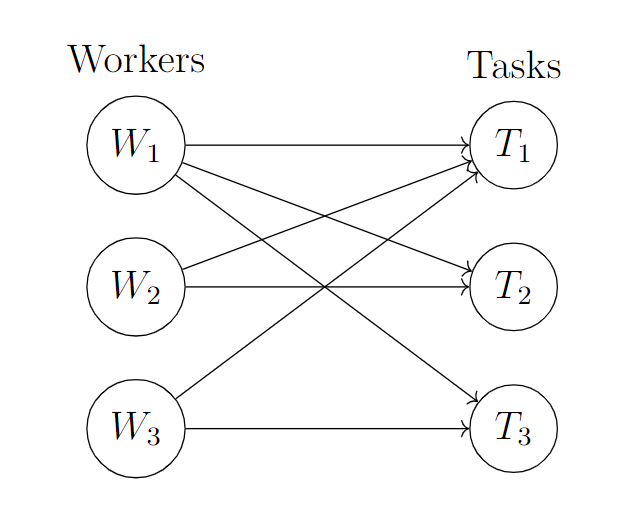
\includegraphics[width=0.6\textwidth]{images/Bipartite_Graph_Assignment_Problem.png}
    \caption{Bipartite Graph for Assignment Problem}
\end{figure}
\FloatBarrier

\textbf{Algorithm Overview}
\FloatBarrier
\begin{algorithm}
\caption{Assignment Problem - Hungarian Algorithm}
\begin{algorithmic}[1]
\item Initialize an \(n \times m\) matrix \(cost\) with the cost of assigning each task to each agent.
\item Subtract the minimum value in each row from all the elements of that row.
\item Subtract the minimum value in each column from all the elements of that column.
\item Initialize an array \(assignment\) of length \(n\) to store the assignment of tasks to agents.
\item Initialize an array \(markedRows\) of length \(n\) and an array \(markedCols\) of length \(m\) with all elements set to False.
\item Find a minimum-cost matching using the Hungarian algorithm.
\end{algorithmic}
\end{algorithm}
\FloatBarrier
\textbf{Python Code}
\FloatBarrier
\begin{lstlisting}
# Python Implementation of Hungarian Algorithm
import numpy as np
from scipy.optimize import linear_sum_assignment

def assignment_problem(cost_matrix):
    row_indices, col_indices = linear_sum_assignment(cost_matrix)
    return list(zip(row_indices, col_indices))

# Example Usage
cost_matrix = np.array([[5, 9, 8], [10, 3, 6], [8, 7, 4]])
assignments = assignment_problem(cost_matrix)
print(assignments)  # Output: [(0, 1), (1, 2), (2, 0)]
\end{lstlisting}
\FloatBarrier

\subsubsection{Formulation as a Network Flow Problem}
The Assignment Problem can be formulated as a network flow problem by constructing a bipartite graph with a source node, a sink node, and edges connecting the source to task nodes and agent nodes to the sink. Each edge has a capacity of 1, representing that each task can only be assigned to one agent. The cost of each assignment is then incorporated into the edge weights.
\FloatBarrier
\begin{figure}[h]
    \centering
    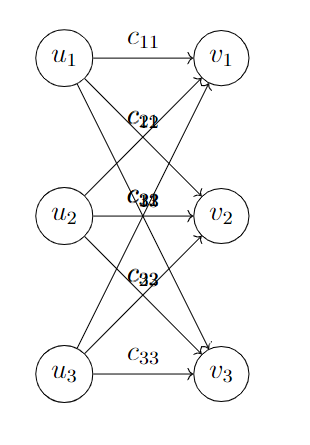
\includegraphics[width=0.6\textwidth]{images/Assignment_Problem_as_Network_Flow.png}
    \caption{Assignment Problem as Network Flow Problem}
\end{figure}
\FloatBarrier

The Assignment Problem formulated as a network flow problem can be solved using the Ford-Fulkerson algorithm or any other maximum flow algorithm. We construct a flow network as described above and compute the maximum flow from the source to the sink. The maximum flow corresponds to the optimal assignment of tasks to agents, and the total cost of the assignment is calculated from the flow and edge weights.

\textbf{Algorithm Overview}
\FloatBarrier
\begin{algorithm}
\caption{Assignment Problem - Network Flow Approach}
\begin{algorithmic}[1]
\item Construct a flow network with a source, a sink, and edges connecting the source to task nodes and agent nodes to the sink, with capacities of 1.
  \item Set the weights of the edges to the costs of assignments.
  \item Compute the maximum flow using a maximum flow algorithm.
  \item Calculate the total cost of the assignment from the flow and edge weights.
\end{algorithmic}
\end{algorithm}
\FloatBarrier
\textbf{Python Code Implementation}
\begin{lstlisting}
# Python Implementation of Network Flow Approach
import networkx as nx
import numpy as np

def assignment_problem_network_flow(cost_matrix):
    num_tasks, num_agents = cost_matrix.shape
    G = nx.DiGraph()
    G.add_node('source', demand=-num_tasks)
    G.add_node('sink', demand=num_tasks)
    
    for i in range(num_tasks):
        G.add_edge('source', f'task_{i}', capacity=1, weight=0)
        for j in range(num_agents):
            G.add_edge(f'task_{i}', f'agent_{j}', capacity=1, weight=cost_matrix[i, j])
    
    for j in range(num_agents):
        G.add_edge(f'agent_{j}', 'sink', capacity=1, weight=0)
    
    flow_dict = nx.min_cost_flow(G)
    assignments = [(task, agent) for agent, flow in flow_dict.items() if agent != 'sink' for task, f in flow.items() if f == 1]
    return assignments

# Example Usage
cost_matrix = np.array([[5, 9, 8], [10, 3, 6], [8, 7, 4]])
assignments = assignment_problem_network_flow(cost_matrix)
print(assignments)  # Output: [('task_0', 'agent_1'), ('task_1', 'agent_2'), ('task_2', 'agent_0')]
\end{lstlisting}
\FloatBarrier

\subsubsection{Solution Approaches}
There are several solution approaches to the Assignment Problem, each with its own advantages and applications.

\textbf{1. Hungarian Algorithm:}
The Hungarian algorithm, also known as the Kuhn-Munkres algorithm, is a combinatorial optimization algorithm that solves the Assignment Problem in polynomial time. It finds the minimum-cost assignment by iteratively selecting the best possible assignment until all tasks are assigned.

\textbf{Algorithm Description:}
The Hungarian algorithm works by iteratively finding augmenting paths in a bipartite graph representation of the assignment problem. It starts with an initial feasible solution and iteratively improves it until an optimal solution is found. At each iteration, the algorithm identifies a set of independent zeros in the cost matrix, constructs a maximal matching, and updates the assignment based on the matching.

\textbf{Mathematical Detail:}
Let \(c_{ij}\) be the cost of assigning task \(i\) to agent \(j\). The algorithm seeks to minimize the total cost of the assignment, which can be represented as the sum of the costs of the assigned tasks:
\[
\text{Total Cost} = \sum_{i=1}^{n} c_{i\pi(i)}
\]
where \(\pi(i)\) represents the agent assigned to task \(i\).

\textbf{Explanation:}
The Hungarian algorithm guarantees an optimal solution to the Assignment Problem in polynomial time. By iteratively selecting augmenting paths, it efficiently finds the minimum-cost assignment without the need for a complex network flow formulation.

\textbf{2. Network Flow Approach:}
The Assignment Problem can also be formulated as a network flow problem, where tasks are nodes on one side of a bipartite graph, agents are nodes on the other side, and edges represent possible assignments with capacities and costs.

\textbf{Algorithm Description:}
In this approach, a flow network is constructed with a source, a sink, and edges connecting the source to task nodes and agent nodes to the sink. Each edge has a capacity of 1, representing that each task can only be assigned to one agent. The cost of each assignment is incorporated into the edge weights. The maximum flow algorithm is then applied to find the optimal assignment.

\textbf{Mathematical Detail:}
Let \(f_{ij}\) be the flow from task \(i\) to agent \(j\) in the flow network. The objective is to maximize the total flow while minimizing the total cost, which can be represented as:
\[
\text{Total Cost} = \sum_{i=1}^{n} \sum_{j=1}^{m} c_{ij} \cdot f_{ij}
\]
subject to flow conservation constraints and capacity constraints.

\textbf{Explanation:}
The network flow approach provides a different perspective on solving the Assignment Problem and allows for the use of standard maximum flow algorithms to find the optimal assignment efficiently.

\textbf{3. Linear Programming Approach:}
Another approach to solving the Assignment Problem is to formulate it as a linear programming problem and use specialized solvers to find the optimal solution.

\textbf{Algorithm Description:}
In this approach, the Assignment Problem is formulated as a linear program with binary decision variables representing the assignment of tasks to agents. The objective function minimizes the total cost of the assignment, subject to constraints ensuring that each task is assigned to exactly one agent and each agent is assigned to at most one task.

\textbf{Mathematical Detail:}
Let \(x_{ij}\) be a binary decision variable representing the assignment of task \(i\) to agent \(j\). The objective function and constraints of the linear program can be formulated as follows:
\[
\text{Minimize} \sum_{i=1}^{n} \sum_{j=1}^{m} c_{ij} \cdot x_{ij}
\]
subject to:
\[
\sum_{j=1}^{m} x_{ij} = 1 \quad \text{for all } i
\]
\[
\sum_{i=1}^{n} x_{ij} \leq 1 \quad \text{for all } j
\]
\[
x_{ij} \in \{0, 1\}
\]

\textbf{Explanation:}
The linear programming approach provides a versatile and generalizable method for solving the Assignment Problem, with the flexibility to incorporate additional constraints and objectives if needed.

\subsection{Network Connectivity and Partitioning}
Network connectivity and partitioning involve analyzing the structure of a network to understand its connectivity properties and partition it into smaller components. These concepts have applications in various fields such as computer networking, social network analysis, and transportation planning.

\subsection{Production Systems and Supply Chains}
Production systems and supply chains involve the efficient management of resources, processes, and logistics to ensure the smooth flow of goods and services from suppliers to consumers. Network flow algorithms play a crucial role in optimizing production systems and supply chains by modeling and solving various optimization problems such as transportation planning, inventory management, and facility location.


\section{Advanced Network Flow Concepts}

\subsection{Minimum Cost Flow Problem}

The Minimum Cost Flow Problem extends the classical maximum flow problem by incorporating costs associated with sending flow through the network. In addition to maximizing the flow from a source to a sink, the objective is to minimize the total cost of sending that flow.

Given a directed graph \(G = (V, E)\) with vertices \(V\) and edges \(E\), where each edge \(e \in E\) has a capacity \(u_e\) and a cost per unit flow \(c_e\), as well as a source node \(s\) and a sink node \(t\), the goal is to find the flow \(f_e\) on each edge \(e\) that maximizes the total flow from \(s\) to \(t\) while minimizing the total cost.

The problem can be formulated as a linear program:

\[
\text{Minimize } \sum_{e \in E} c_e \cdot f_e
\]
\[
\text{subject to:}
\]
\[
\sum_{e \in \delta^-(v)} f_e - \sum_{e \in \delta^+(v)} f_e = 
\begin{cases} 
1 & \text{if } v = s \\
-1 & \text{if } v = t \\
0 & \text{otherwise}
\end{cases}
\]
\[
0 \leq f_e \leq u_e \text{ for all } e \in E
\]

Here, \(\delta^-(v)\) and \(\delta^+(v)\) represent the set of incoming and outgoing edges of vertex \(v\), respectively.


The Minimum Cost Flow Problem can be solved using the successive shortest path algorithm, which is an extension of the Ford-Fulkerson algorithm. It iteratively finds the shortest augmenting path in terms of cost from the source to the sink and adjusts the flow along that path.

The algorithm maintains a flow and a potential function. The flow represents the current flow on each edge, while the potential function assigns a cost to each vertex. At each iteration, the algorithm finds the shortest augmenting path using Dijkstra's algorithm with edge costs adjusted by the potential function. It then updates the flow along this path and adjusts the potential function accordingly.

The pseudocode for the successive shortest path algorithm is as follows:
\FloatBarrier
\begin{list}{}{\leftmargin=1em \itemindent=0em}
\item \textbf{Algorithm:} Successive Shortest Path Algorithm
\item \textbf{Initialization:} 
\begin{enumerate}
\item Initialize flow $f_e$ on each edge $e \in E$ to 0
\item Initialize potential $\pi_v$ for each vertex $v \in V$
\end{enumerate}
\item \textbf{While} there exists an augmenting path from $s$ to $t$, do:
\begin{enumerate}
\item Find the shortest augmenting path using Dijkstra's algorithm with adjusted edge costs
\item Update the flow along the augmenting path
\item Update the potential function based on the shortest path tree
\end{enumerate}
\end{list}
\FloatBarrier
The edge costs used in Dijkstra's algorithm are adjusted based on the potential function: \(c'_e = c_e + \pi_{v_i} - \pi_{v_j}\), where \(v_i\) and \(v_j\) are the vertices incident to edge \(e\).

Here's the Python implementation of the successive shortest path algorithm for solving the Minimum Cost Flow Problem:
\FloatBarrier
\begin{lstlisting}
def successive_shortest_path(graph, source, sink):
    initialize_flow(graph)
    initialize_potential(graph)
    while augmenting_path_exists(graph, source, sink):
        shortest_path = dijkstra_shortest_path(graph, source, sink)
        update_flow(graph, shortest_path)
        update_potential(graph, shortest_path)
    return total_flow, total_cost
\end{lstlisting}
\FloatBarrier

\subsection{Multi-commodity Flow Problems}

Multi-commodity Flow Problems involve multiple commodities flowing through a network simultaneously, each with its own source and sink nodes and flow requirements. The objective is to find flow assignments for each commodity that satisfy their respective demands while respecting capacity constraints and minimizing the total cost.

Given a directed graph \(G = (V, E)\) with vertices \(V\) and edges \(E\), and a set of commodities \(K\), where each commodity \(k \in K\) has a source node \(s_k\) and a sink node \(t_k\), as well as a flow demand \(d_k\), capacity \(u_e\), and cost per unit flow \(c_e\), the goal is to find flow assignments \(f_{ek}\) for each commodity \(k\) such that:

\[
\sum_{k \in K} f_{ek} = 0 \text{ for all } e \in E \setminus \{(s_k, t_k)\}
\]
\[
\sum_{e \in \delta^-(v)} f_{ek} - \sum_{e \in \delta^+(v)} f_{ek} = 
\begin{cases} 
d_k & \text{if } v = s_k \\
-d_k & \text{if } v = t_k \\
0 & \text{otherwise}
\end{cases}
\]
\[
0 \leq f_{ek} \leq u_e \text{ for all } e \in E, k \in K
\]

The Multi-commodity Flow Problem can be solved using the successive shortest path algorithm with capacity scaling, which is an extension of the successive shortest path algorithm for single-commodity flow problems. It iteratively finds augmenting paths for each commodity and adjusts the flow along those paths.

The algorithm maintains a flow for each commodity and a scaling factor that gradually increases to improve efficiency. At each iteration, the algorithm finds shortest augmenting paths for each commodity using Dijkstra's algorithm with adjusted edge costs and capacities. It then updates the flow along these paths and adjusts the scaling factor accordingly.

The pseudocode for the successive shortest path algorithm with capacity scaling is similar to Algorithm \ref{alg:ssp}, with additional steps to handle multiple commodities and scaling:
\FloatBarrier
\begin{list}{}{\leftmargin=1em \itemindent=0em}
\item \textbf{Algorithm:} Successive Shortest Path Algorithm with Capacity Scaling
\item \textbf{Initialization:} 
\begin{enumerate}
\item Initialize flow $f_{ek}$ on each edge $e \in E$ for each commodity $k \in K$ to 0
\item Initialize scaling factor $f_{\text{scale}}$ to 1
\end{enumerate}
\item \textbf{While} there exists an augmenting path for any commodity, do:
\begin{enumerate}
\item Find the shortest augmenting path for each commodity using Dijkstra's algorithm with adjusted edge costs and capacities
\item Update the flow along the augmenting paths for each commodity
\item Update the scaling factor based on the maximum flow increase
\end{enumerate}
\end{list}
\FloatBarrier
The edge costs and capacities used in Dijkstra's algorithm are adjusted based on the flow and the scaling factor: \(c'_{ek} = \frac{c_{ek}}{f_{\text{scale}}}\) and \(u'_{ek} = \frac{u_{ek}}{f_{\text{scale}}}\).

Here's the Python implementation of the successive shortest path algorithm with capacity scaling for solving Multi-commodity Flow Problems:

\begin{lstlisting}
def successive_shortest_path_with_scaling(graph, commodities):
    initialize_flow(graph, commodities)
    scaling_factor = 1
    while augmenting_path_exists(graph, commodities):
        shortest_paths = dijkstra_shortest_paths(graph, commodities)
        update_flow(graph, shortest_paths)
        scaling_factor *= 2
    return total_flow, total_cost
\end{lstlisting}
\FloatBarrier

\subsection{Dynamic Network Flow Problems}

Dynamic Network Flow Problems involve flow networks where the capacities and demands may change over time. The goal is to dynamically adjust the flow in response to changing conditions while minimizing costs or maximizing efficiency.

Given a sequence of time periods \(T\), where each time period \(t \in T\) has its own set of capacities \(u_{et}\) and demands \(d_{kt}\), the objective is to find flow assignments \(f_{ekt}\) for each time period \(t\) that satisfy the demands while respecting capacity constraints and minimizing the total cost.

The problem can be formulated similarly to the single-commodity flow problem, with additional constraints and variables for each time period:

\[
\text{Minimize } \sum_{t \in T} \sum_{e \in E} c_{et} \cdot f_{et}
\]
\[
\text{subject to:}
\]
\[
\sum_{e \in \delta^-(v)} f_{et} - \sum_{e \in \delta^+(v)} f_{et} = 
\begin{cases} 
d_{kv} & \text{if } v = s_k \\
-d_{kv} & \text{if } v = t_k \\
0 & \text{otherwise}
\end{cases}
\]
\[
0 \leq f_{et} \leq u_{et} \text{ for all } e \in E, t \in T
\]

The Dynamic Network Flow Problem can be solved using a rolling horizon approach, where flow assignments are made for each time period individually, taking into account the changing capacities and demands.

At each time period \(t\), the algorithm solves a single-commodity flow problem with the current capacities and demands. This can be done using any suitable flow algorithm, such as the successive shortest path algorithm. The algorithm then moves to the next time period and repeats the process until all time periods have been considered.

The pseudocode for the rolling horizon approach is as follows:
\FloatBarrier
\begin{list}{}{\leftmargin=1em \itemindent=0em}
\item \textbf{Algorithm:} Rolling Horizon Approach for Dynamic Network Flow
\item \textbf{Input:} Graph, Capacities, Demands
\item \textbf{Output:} Updated capacities and demands
\end{list}
\begin{enumerate}
\item For each time period $t \in T$:
\begin{enumerate}
\item Solve the single-commodity flow problem for time period $t$
\item Update the capacities and demands for the next time period
\end{enumerate}
\end{enumerate}
\FloatBarrier

Here's the Python implementation of the rolling horizon approach for solving Dynamic Network Flow Problems:
\FloatBarrier
\begin{lstlisting}
def rolling_horizon_approach(graph, capacities, demands):
    for time_period, (capacity, demand) in enumerate(zip(capacities, demands)):
        solve_single_commodity_flow(graph, capacity, demand)
        update_capacities_and_demands(graph, capacities[time_period + 1], demands[time_period + 1])
\end{lstlisting}
\FloatBarrier

\section{Software and Tools for Network Flow Analysis}

Network flow analysis requires a range of software tools for modeling, analyzing, and visualizing flow networks. These tools vary from commercial software packages to open-source libraries and APIs.

\subsection{Commercial and Open Source Software}

\textbf{Commercial Software:} Several commercial software packages provide comprehensive network flow analysis capabilities, including optimization, visualization, and simulation. Examples include MATLAB's Optimization Toolbox, IBM ILOG CPLEX Optimization Studio, and LINDO Systems' LINDO API.

\textbf{Open Source Software:} Open-source alternatives are widely used for network flow analysis due to their flexibility and cost-effectiveness. Popular open-source software includes GNU Octave, Scilab, and R, which provide extensive libraries and packages for optimization and network analysis.

\subsection{Libraries and APIs for Development}

Libraries and APIs offer developers the flexibility to integrate network flow analysis into their own applications and workflows.

\textbf{NetworkX:} NetworkX is a Python library for the creation, manipulation, and study of complex networks. It provides algorithms for network flow analysis, graph theory, and visualization, making it a popular choice for network analysis tasks.

\textbf{Pyomo:} Pyomo is a Python-based open-source optimization modeling language that supports a diverse range of optimization problem types, including network flow problems. It integrates with solvers such as GLPK and CBC to solve optimization models efficiently.

\subsection{Simulation and Visualization Tools}

Simulation and visualization tools are essential for understanding and communicating the results of network flow analysis.

\textbf{Gephi:} Gephi is an open-source network visualization tool that allows users to explore and analyze large-scale networks. It provides interactive visualization features for exploring network structure, flow dynamics, and community detection.

\textbf{MATLAB/Simulink:} MATLAB and Simulink offer powerful simulation and modeling capabilities for analyzing network flow dynamics. With built-in functions and toolboxes for optimization and simulation, MATLAB/Simulink is widely used in academic and industrial settings for network flow analysis.

\textbf{Python with Matplotlib and NetworkX:} Python, combined with libraries such as Matplotlib for visualization and NetworkX for network analysis, provides a flexible and customizable platform for simulating and visualizing network flow dynamics.

\FloatBarrier
\subsubsection{Python Example using NetworkX}

Below is a Python example demonstrating how to model a flow network using NetworkX and visualize it using Matplotlib:

\begin{lstlisting}
import networkx as nx
import matplotlib.pyplot as plt

# Create a directed graph
G = nx.DiGraph()

# Add nodes
G.add_nodes_from(['s', 'a', 'b', 't'])

# Add edges with capacities
G.add_edge('s', 'a', capacity=10)
G.add_edge('s', 'b', capacity=5)
G.add_edge('a', 'b', capacity=15)
G.add_edge('a', 't', capacity=10)
G.add_edge('b', 't', capacity=10)

# Visualize the flow network
pos = nx.spring_layout(G)  # positions for all nodes
nx.draw_networkx_nodes(G, pos, node_size=700)
nx.draw_networkx_edges(G, pos)
nx.draw_networkx_labels(G, pos)
nx.draw_networkx_edge_labels(G, pos, edge_labels=nx.get_edge_attributes(G, 'capacity'))
plt.axis('off')
plt.show()
\end{lstlisting}
\FloatBarrier

The above Python code creates a flow network with nodes 's', 'a', 'b', and 't', and edges with capacities. It then visualizes the flow network using NetworkX and Matplotlib, displaying the nodes, edges, and edge capacities.


\section{Case Studies and Real-World Examples}

\subsection{Transportation and Logistics}
Transportation and logistics networks are prime examples of applications where network flow algorithms play a crucial role. These networks involve the movement of goods, people, or information from one location to another, often with constraints on capacities, costs, and time.

One common problem in transportation and logistics is the \textbf{minimum cost flow} problem, which seeks to find the most cost-effective way to transport goods from suppliers to consumers given various constraints. Mathematically, the problem can be formulated as follows:

Given a directed graph \(G = (V, E)\) representing the transportation network, where \(V\) is the set of nodes (representing suppliers, consumers, and intermediate locations) and \(E\) is the set of edges (representing transportation routes), and each edge \(e \in E\) has a capacity \(u_e\) and a cost per unit flow \(c_e\), find the flow \(f_{ij}\) from each source node \(i\) to each sink node \(j\) that minimizes the total cost while satisfying the capacity constraints and flow conservation at each node.

The mathematical formulation can be represented as a linear program:

\[
\begin{aligned}
\text{minimize} \quad & \sum_{e \in E} c_e \cdot f_e \\
\text{subject to} \quad & \sum_{e \in \delta^-(v)} f_e - \sum_{e \in \delta^+(v)} f_e = b_v, \quad \forall v \in V \\
& 0 \leq f_e \leq u_e, \quad \forall e \in E
\end{aligned}
\]

where \(f_e\) is the flow on edge \(e\), \(\delta^-(v)\) and \(\delta^+(v)\) represent the set of incoming and outgoing edges of node \(v\) respectively, and \(b_v\) represents the supply (for suppliers) or demand (for consumers) at node \(v\).

Here's a Python implementation of the Ford-Fulkerson algorithm to solve the minimum cost flow problem:
\FloatBarrier
\begin{lstlisting}
# Ford-Fulkerson Algorithm for Minimum Cost Flow
def ford_fulkerson(graph, source, sink):
    # Initialize flow to zero
    flow = {(u, v): 0 for u, v in graph.edges()}
    
    # Repeat until no augmenting path exists
    while True:
        # Find augmenting path using BFS
        path = find_augmenting_path(graph, source, sink)
        if not path:
            break
        
        # Determine augmenting flow
        augmenting_flow = min(graph[u][v]['capacity'] - flow[u, v] for u, v in path)
        
        # Update flow along the path
        for u, v in path:
            flow[u, v] += augmenting_flow
            flow[v, u] -= augmenting_flow
    
    return flow
\end{lstlisting}
\FloatBarrier

\subsection{Telecommunications Networks}
Telecommunications networks involve the transmission of data, voice, and video signals between various nodes such as routers, switches, and endpoints. Network flow algorithms are used in optimizing data routing, resource allocation, and traffic management in these networks.


A common problem in telecommunications networks is the \textbf{maximum flow} problem, which seeks to determine the maximum amount of data that can be transmitted from a source node to a destination node through the network. Mathematically, the problem can be formulated as follows:

Given a directed graph \(G = (V, E)\) representing the telecommunication network, where \(V\) is the set of nodes (representing routers, switches, and endpoints) and \(E\) is the set of edges (representing communication links), and each edge \(e \in E\) has a capacity \(u_e\), find the maximum flow \(f_{\text{max}}\) from a source node \(s\) to a destination node \(t\) while satisfying the capacity constraints and flow conservation at each node.

The mathematical formulation can be represented as a linear program:

\[
\begin{aligned}
\text{maximize} \quad & f_{st} \\
\text{subject to} \quad & \sum_{e \in \delta^-(v)} f_e - \sum_{e \in \delta^+(v)} f_e = 0, \quad \forall v \in V \setminus \{s, t\} \\
& \sum_{e \in \delta^-(s)} f_e - \sum_{e \in \delta^+(s)} f_e = -f_{\text{max}} \\
& \sum_{e \in \delta^-(t)} f_e - \sum_{e \in \delta^+(t)} f_e = f_{\text{max}} \\
& 0 \leq f_e \leq u_e, \quad \forall e \in E
\end{aligned}
\]

where \(f_e\) is the flow on edge \(e\), \(\delta^-(v)\) and \(\delta^+(v)\) represent the set of incoming and outgoing edges of node \(v\) respectively, and \(f_{st}\) represents the maximum flow from \(s\) to \(t\).

Here's a Python implementation of the Edmonds-Karp algorithm to solve the maximum flow problem:
\FloatBarrier
\begin{lstlisting}
# Edmonds-Karp Algorithm for Maximum Flow
def edmonds_karp(graph, source, sink):
    flow = {(u, v): 0 for u, v in graph.edges()}
    residual_graph = graph.copy()
    max_flow = 0
    
    while True:
        # Find augmenting path using BFS
        path = find_augmenting_path(residual_graph, source, sink)
        if not path:
            break
        
        # Determine augmenting flow
        augmenting_flow = min(residual_graph[u][v]['capacity'] - flow[u, v] for u, v in path)
        
        # Update flow along the path
        for u, v in path:
            flow[u, v] += augmenting_flow
            flow[v, u] -= augmenting_flow
        
        max_flow += augmenting_flow
    
    return max_flow, flow
\end{lstlisting}
\FloatBarrier

\subsection{Energy Distribution Networks}
Energy distribution networks, such as electrical grids and pipelines, involve the transmission of energy (electricity, gas, etc.) from producers to consumers. Network flow algorithms are used in optimizing energy routing, load balancing, and fault detection in these networks.

In energy distribution networks, one important problem is the \textbf{minimum cost flow} problem, which seeks to minimize the cost of transmitting energy from producers to consumers while satisfying various constraints. Mathematically, the problem can be formulated similarly to the minimum cost flow problem in transportation networks.

\[
\begin{aligned}
\text{minimize} \quad & \sum_{e \in E} c_e \cdot f_e \\
\text{subject to} \quad & \sum_{e \in \delta^-(v)} f_e - \sum_{e \in \delta^+(v)} f_e = b_v, \quad \forall v \in V \\
& 0 \leq f_e \leq u_e, \quad \forall e \in E
\end{aligned}
\]

where \(f_e\) is the flow on edge \(e\), \(\delta^-(v)\) and \(\delta^+(v)\) represent the set of incoming and outgoing edges of node \(v\) respectively, and \(b_v\) represents the supply (energy production) or demand (energy consumption) at node \(v\).

Here's a Python implementation of the Push-Relabel algorithm to solve the minimum cost flow problem in energy distribution networks:
\FloatBarrier
\begin{lstlisting}
# Push-Relabel Algorithm for Minimum Cost Flow
def push_relabel(graph, source, sink):
    # Initialize preflow and heights
    preflow = {(u, v): 0 for u, v in graph.edges()}
    height = {v: 0 for v in graph.nodes()}
    excess = {v: 0 for v in graph.nodes()}
    
    # Initialize preflow from source
    for v in graph.successors(source):
        preflow[source, v] = graph[source][v]['capacity']
        excess[v] += graph[source][v]['capacity']
    
    # Push-relabel operations
    while True:
        v = find_node_with_excess(graph, excess)
        if not v:
            break
        push_relabel_operation(graph, preflow, height, excess, v)
    
    # Calculate total flow and return preflow
    total_flow = sum(preflow[source, v] for v in graph.successors(source))
    return total_flow, preflow
\end{lstlisting}
\FloatBarrier

\section{Challenges and Future Directions}
Network flow analysis has made significant strides in various domains, but several challenges remain, and there are exciting future directions to explore.

\subsection{Scalability and Large-Scale Applications}
One of the primary challenges in network flow analysis is scalability, especially in large-scale applications such as transportation networks, communication networks, and social networks. As networks continue to grow in size and complexity, traditional algorithms may struggle to handle the sheer volume of data and the intricacies of real-world networks. Future research efforts should focus on developing scalable algorithms and techniques capable of efficiently handling massive networks.

\subsection{Integrating Machine Learning with Network Flow Analysis}
Another promising direction is the integration of machine learning techniques with network flow analysis. Machine learning models can complement traditional algorithms by providing insights into network behavior, predicting flow patterns, and optimizing network performance. For example, neural networks can be trained to predict traffic flow in transportation networks or detect anomalies in communication networks. Integrating machine learning with network flow analysis opens up new possibilities for automated decision-making and optimization in various applications.

Let's consider the \textbf{Shortest Path Algorithm}, a fundamental algorithm in network flow analysis:

The Shortest Path Algorithm is used to find the shortest path between two nodes in a weighted graph. It can be applied to various network flow problems, such as finding the shortest route in transportation networks or the minimum delay path in communication networks. Here's how the algorithm works:
\FloatBarrier
\begin{algorithm}[H]
\caption{Shortest Path Algorithm}
\begin{algorithmic}[1]
\Procedure{ShortestPath}{$G, s, t$}
    \State Initialize distances $dist[v]$ for all nodes $v$ in $G$ to $\infty$
    \State Set $dist[s] = 0$
    \State Initialize priority queue $Q$
    \State Insert $s$ into $Q$ with priority $0$
    \While{$Q$ is not empty}
        \State Extract node $u$ with minimum distance from $Q$
        \For{each neighbor $v$ of $u$}
            \If{$dist[u] + weight(u, v) < dist[v]$}
                \State $dist[v] = dist[u] + weight(u, v)$
                \State Update priority of $v$ in $Q$
            \EndIf
        \EndFor
    \EndWhile
    \State \textbf{return} $dist[t]$
\EndProcedure
\end{algorithmic}
\end{algorithm}
\FloatBarrier
Let \(G\) be a weighted graph with nodes \(s\) and \(t\) representing the source and sink, respectively. The algorithm computes the shortest distance \(dist[v]\) from \(s\) to every other node \(v\) in the graph. The priority queue \(Q\) is used to efficiently select the node with the minimum distance at each iteration.

Here's a Python implementation of the Shortest Path Algorithm using the priority queue implementation from the heapq module:
\FloatBarrier
\begin{lstlisting}
import heapq

def shortest_path(graph, source, target):
    distances = {node: float('inf') for node in graph}
    distances[source] = 0
    pq = [(0, source)]

    while pq:
        current_distance, current_node = heapq.heappop(pq)

        if current_distance > distances[current_node]:
            continue

        for neighbor, weight in graph[current_node].items():
            distance = current_distance + weight
            if distance < distances[neighbor]:
                distances[neighbor] = distance
                heapq.heappush(pq, (distance, neighbor))

    return distances[target]
\end{lstlisting}
\FloatBarrier

\subsection{Theoretical Advances and Open Problems}
In addition to scalability and machine learning integration, there are several theoretical advances and open problems in network flow analysis. These include:
\begin{itemize}
    \item Developing approximation algorithms for NP-hard network flow problems.
    \item Investigating the resilience and robustness of network flow algorithms to node and edge failures.
    \item Exploring the application of network flow analysis in emerging fields such as blockchain networks and Internet of Things (IoT) systems.
    \item Studying the impact of dynamic and uncertain environments on network flow optimization.
\end{itemize}
Addressing these challenges and advancing the theoretical foundations of network flow analysis will pave the way for innovative solutions in various domains.


\section{Conclusion}

\subsection{Recap of Key Points}
This discussion has provided a comprehensive look at network flow analysis, specifically focusing on algorithms such as Ford-Fulkerson and Push-Relabel that solve maximum flow problems. Starting with the basics of the maximum flow problem and its real-world significance, we've seen how these algorithms optimize resource flow in networks ranging from transportation to data communication. The Ford-Fulkerson algorithm enhances network flow through augmenting paths, while the Push-Relabel algorithm optimizes it by maintaining a preflow and adjusting locally for maximum efficiency.

The examination of these methods underscores the role of network flow analysis in enhancing system efficiencies across various sectors, pinpointing both the opportunities and challenges presented by maximum flow problems.

\subsection{The Broad Impact of Network Flow Analysis}
Network flow analysis profoundly influences several domains, facilitating improved decision-making and resource management. It is instrumental in fields such as transportation planning, where it helps minimize traffic congestion, and in supply chain management, where it ensures efficient distribution and cost management.

In technology, network flow is pivotal in optimizing computer network operations by improving data routing protocols, which enhances communication network reliability and performance. Beyond these applications, network flow principles are also integrated into financial models for risk management, telecommunication systems for service quality, healthcare systems for patient management, and energy sectors for optimizing power distribution.

The pervasive influence of network flow analysis across these diverse fields highlights its critical role in modern society, driving advancements that contribute to economic stability, environmental sustainability, and overall societal progress.




\section{Exercises and Problems}

In this section, we provide a variety of exercises and problems aimed at reinforcing your understanding of network flow algorithm techniques. These exercises cover both conceptual questions to test your understanding and practical coding problems to strengthen your skills. 

\subsection{Conceptual Questions to Test Understanding}

Below are conceptual questions designed to test your understanding of network flow algorithm techniques:

\begin{itemize}
    \item Explain the concept of a flow network and its components.
    \item What is the maximum flow problem, and how is it different from other network flow problems?
    \item Describe the Ford-Fulkerson algorithm and its basic steps.
    \item What is the significance of residual networks in the context of network flow algorithms?
    \item Explain the concept of augmenting paths and their role in finding the maximum flow.
    \item How does the Edmonds-Karp algorithm improve upon the Ford-Fulkerson algorithm?
    \item Discuss the applications of network flow algorithms in real-world scenarios.
    \item What are some common optimization techniques used in network flow algorithms?
\end{itemize}

\subsection{Practical Coding Problems to Strengthen Skills}

Now, let's dive into practical coding problems related to network flow techniques. Solve these problems to enhance your skills in implementing and applying network flow algorithms:

\begin{itemize}
    \item \textbf{Problem 1:} Implement the Ford-Fulkerson algorithm to find the maximum flow in a given flow network.
    
    \begin{algorithm}
    \caption{Ford-Fulkerson Algorithm}\label{ford-fulkerson}
    \begin{algorithmic}[1]
    \Procedure{FordFulkerson}{Graph $G$, Node $s$, Node $t$}
    \State Initialize flow $f$ to 0
    \While{there exists an augmenting path $p$ from $s$ to $t$ in residual network $G_f$}
    \State Find the bottleneck capacity $c_f(p)$ of path $p$
    \State Update the flow $f$ by adding $c_f(p)$ along path $p$
    \State Update the residual capacities of edges in $G_f$
    \EndWhile
    \State \textbf{return} flow $f$
    \EndProcedure
    \end{algorithmic}
    \end{algorithm}
    
    
    \item \textbf{Problem 2:} Implement the Edmonds-Karp algorithm to find the maximum flow in a given flow network.
    
    \begin{algorithm}
    \caption{Edmonds-Karp Algorithm}\label{edmonds-karp}
    \begin{algorithmic}[1]
    \Procedure{EdmondsKarp}{Graph $G$, Node $s$, Node $t$}
    \State Initialize flow $f$ to 0
    \While{there exists a shortest augmenting path $p$ from $s$ to $t$ in residual network $G_f$}
    \State Find the bottleneck capacity $c_f(p)$ of path $p$
    \State Update the flow $f$ by adding $c_f(p)$ along path $p$
    \State Update the residual capacities of edges in $G_f$
    \EndWhile
    \State \textbf{return} flow $f$
    \EndProcedure
    \end{algorithmic}
    \end{algorithm}
    
    \FloatBarrier
    
    
    \item \textbf{Problem 3:} Implement the Dinic's algorithm to find the maximum flow in a given flow network.
    
    \item \textbf{Problem 4:} Given a flow network with capacities on edges, implement an algorithm to find the maximum flow and minimum cut.
    
    \item \textbf{Problem 5:} Apply network flow techniques to solve a real-world transportation problem, such as the maximum flow problem in traffic networks or supply chain optimization.
\end{itemize}

These practical problems, along with their algorithmic descriptions and Python code implementations, will help solidify your understanding and mastery of network flow algorithm techniques.

\section{Further Reading and Resources}

In addition to the concepts covered in this course, there are plenty of resources available for further exploration of Network Flow algorithms. Below are some key textbooks, papers, online courses, tutorials, and software resources to enhance your understanding and implementation of Network Flow algorithms.

\subsection{Key Textbooks and Papers}

Network Flow algorithms have been extensively studied and documented in various textbooks and research papers. Here are some essential readings that provide in-depth coverage of the topic:

\begin{itemize}
    \item \textbf{Introduction to Algorithms} by Thomas H. Cormen, Charles E. Leiserson, Ronald L. Rivest, and Clifford Stein: This widely-used textbook covers Network Flow algorithms in detail, providing both theoretical foundations and practical implementation insights.
    \item \textbf{Network Flows: Theory, Algorithms, and Applications} by Ravindra K. Ahuja, Thomas L. Magnanti, and James B. Orlin: This comprehensive book offers a thorough treatment of Network Flow algorithms, including advanced topics such as multi-commodity flows and network design.
    \item \textbf{Ford-Fulkerson Algorithm} by L.R. Ford Jr. and D.R. Fulkerson: This seminal paper introduces the Ford-Fulkerson algorithm for solving the maximum flow problem, laying the groundwork for subsequent research in Network Flow algorithms.
\end{itemize}

\subsection{Online Courses and Tutorials}

If you prefer online learning, there are several courses and tutorials available that cover Network Flow algorithms. These resources offer video lectures, interactive exercises, and real-world examples to help you grasp the concepts effectively:

\begin{itemize}
    \item \textbf{Coursera - Algorithms Specialization} by Stanford University: This specialization includes a course on Graph Search, Shortest Paths, and Data Structures, which covers Network Flow algorithms along with other graph algorithms.
    \item \textbf{edX - Algorithm Design and Analysis} by Massachusetts Institute of Technology (MIT): This course covers advanced algorithms, including Network Flow algorithms, and provides a deep dive into algorithmic design principles.
    \item \textbf{YouTube - Network Flow Algorithms Playlist} by William Fiset: This series of video tutorials offers comprehensive explanations of various Network Flow algorithms, including Ford-Fulkerson, Edmonds-Karp, and Dinic's algorithm.
\end{itemize}

\subsection{Software and Coding Resources}

Implementing Network Flow algorithms requires suitable software tools and libraries. Fortunately, there are several open-source software resources available that facilitate the implementation and experimentation of Network Flow algorithms:

\begin{itemize}
    \item \textbf{NetworkX}: NetworkX is a Python library for the creation, manipulation, and study of complex networks. It provides implementations of various Network Flow algorithms, making it a valuable resource for algorithm development and analysis.
    
    \item \textbf{PyFlow}: PyFlow is a Python library that specializes in solving network flow problems. It offers efficient implementations of classic algorithms such as Ford-Fulkerson and Edmonds-Karp, as well as more advanced techniques like push-relabel and preflow-push.
    
    \item \textbf{Optimization Toolbox in MATLAB}: MATLAB's Optimization Toolbox includes functions for solving optimization problems, including linear programming (LP) and mixed-integer linear programming (MILP) problems. These tools can be used to formulate and solve Network Flow problems efficiently.
\end{itemize}

These resources provide a solid foundation for further study and exploration of Network Flow algorithms. Whether you prefer textbooks, online courses, or hands-on coding, there are plenty of options available to deepen your understanding and expertise in this fascinating field.
\end{document}